\section{Introdução}

% Emoção/sentimentos/opiniões em arte.

Grande quantidade dos textos produzidos pelos seres humanos tem como
objetivo refletirem as opiniões e sentimentos do autor, em contraste
com a categoria de textos onde a preocupação é com fatos e expressões
objetivas. Dentro dos textos subjetivos, aqueles de cunho artístico sempre foram exemplo mais notável de expressividade emocional
\cite{PJA57}.

% Expressividade em música.

Uma das formas de arte mais antigas, a música consegue alcançar
níveis de expressividade emocional especialmente interessantes, 
combinando tanto a linguagem natural quanto sua própria linguagem
através de ritmo, sons, instrumentos, entre outros elementos. Sendo
dotada de tal capacidade de expressão, a música foi e continua
sendo estudada por cientistas da área da psicologia
\cite{juslin2001music}. Dentre os 
vários aspectos que relacionam música e emoção, três deles são
particularmente instigantes para serem estudados:

\begin{itemize}
	\item Como emoções podem influenciar a música que alguém escolhe
	ouvir.
	\item Como música pode expressar emoção e sentimentos.
	\item Como música pode induzir emoções no ouvinte. 
\end{itemize}

\begin{figure}
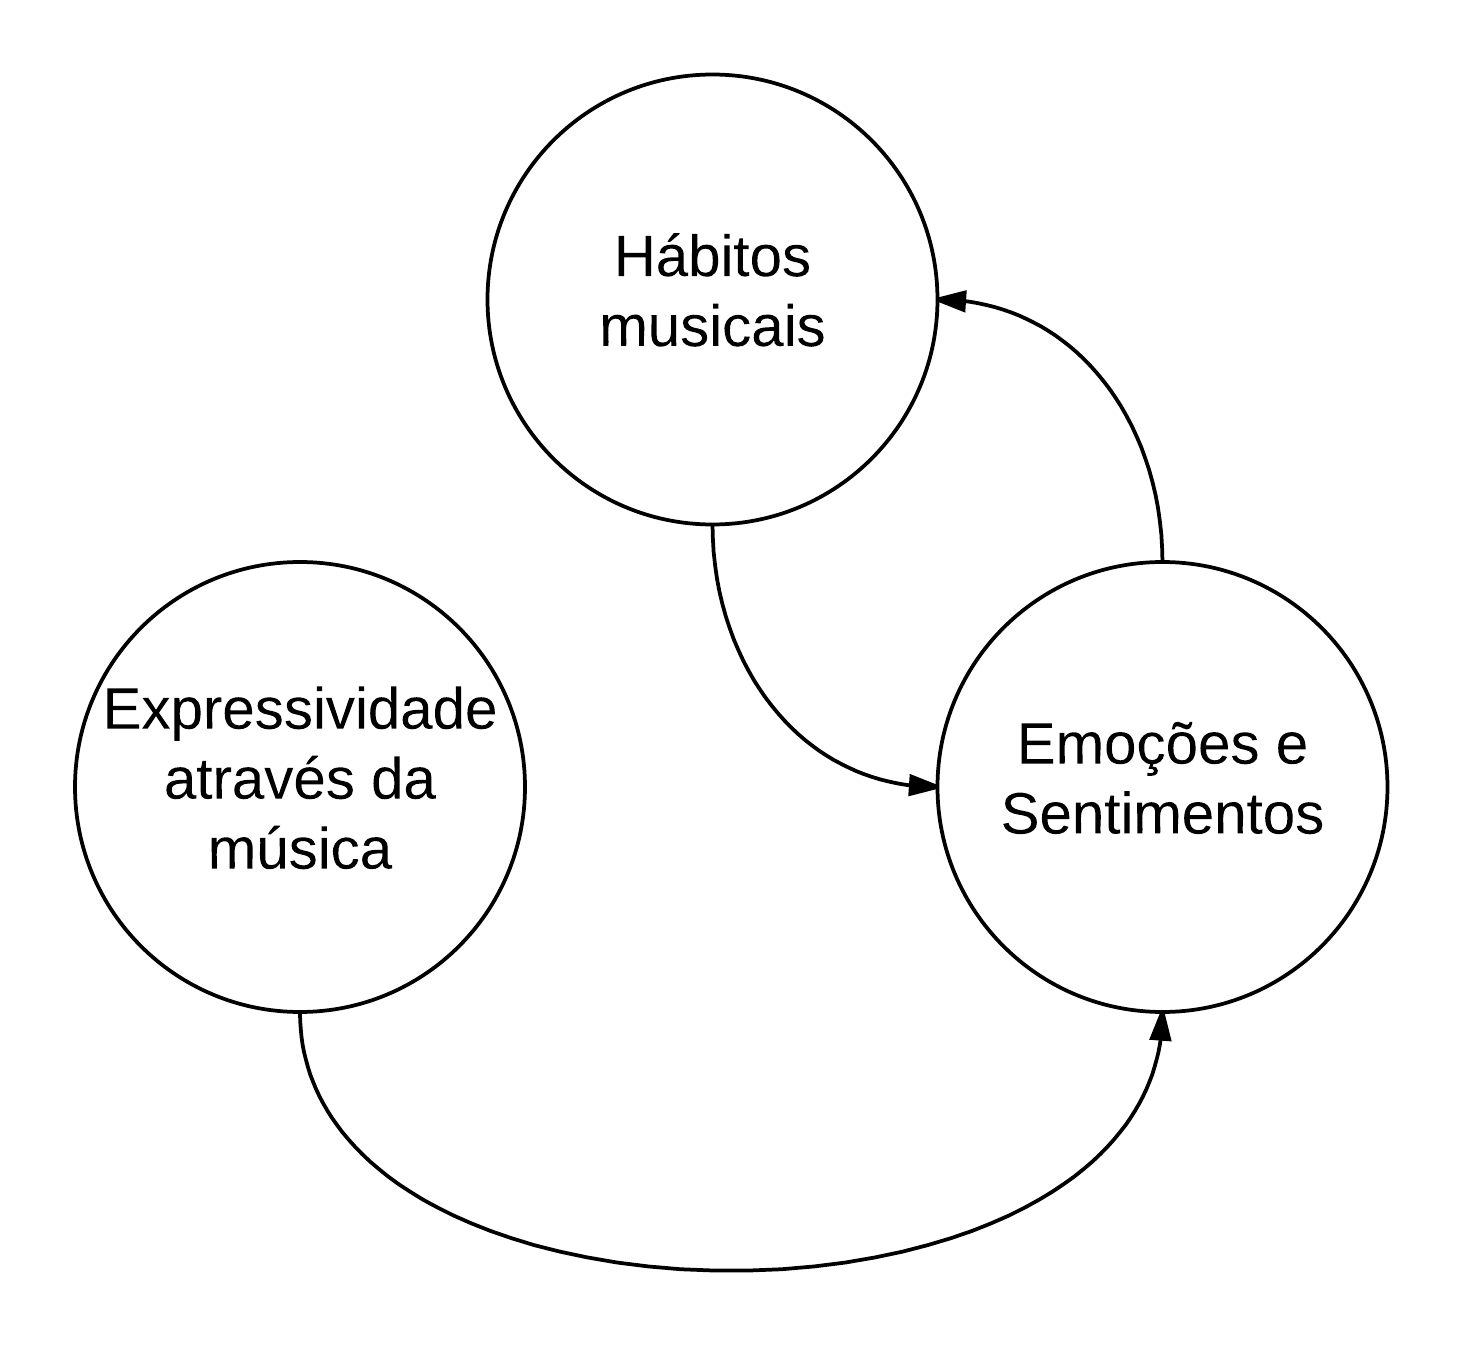
\includegraphics[height=3in, width=3in]{music-mood.png}
\caption{Relação entre expressividade de um artista através de sua música
	e o ciclo criado entre a indução de sentimentos no ouvinte e a escolha
	por músicas que correspondem a seu humor atual.}
\label{fig:music-mood}
\end{figure}

% Música como reflexo das emoções do ouvinte.
% Consumo massivo de música na modernidade - dados/estudo relevantes.
Já sabemos que os hábitos musicais de uma pessoa influenciam diretamente
seu humor, sentimentos e emoções \cite{mccraty1998}. Esse aspecto, aliado ao fato de que o consumo de música (...) nos fornece grande indicação de que podemos
utilizar os hábitos musicais de um ouvinte como fonte de informações a
respeito do humor e emoções do mesmo.

\section{Problema}

\section{Modelagem}

\section{Implementação}

\section{Estudo de caso}

\section{Conclusão}